% This is LLNCS.DEM the demonstration file of
% the LaTeX macro package from Springer-Verlag
% for Lecture Notes in Computer Science,
% version 2.4 for LaTeX2e as of 16. April 2010
%

\documentclass{llncs}
\usepackage{amsmath}
\usepackage{amsfonts}
\usepackage{amssymb}
\usepackage{german}
\usepackage{tabularx}
\usepackage[pdftex]{graphicx}
\usepackage{wrapfig}
\usepackage[utf8]{inputenc}
\usepackage[T1]{fontenc}
\usepackage{makeidx}  % allows for indexgeneration
\usepackage{caption}
\usepackage{tikz}
\usetikzlibrary{shapes,arrows}
%%%<
\usepackage{verbatim}
%\usepackage[active,tightpage]{preview}
%\PreviewEnvironment{tikzpicture}
%\setlength\PreviewBorder{5pt}%
%
\begin{document}
%
\mainmatter              % start of the contributions
%
\title{Rezept für Welfencreme, erweitert als timed Net}
%
\titlerunning{Formale Simulation und Verifikation verteilter Algorithmen SS17}  % abbreviated title (for running head)
%                                     also used for the TOC unless
%                                     \toctitle is used
%
\author{Jan Scholz, Lukas Kozlowski}
%
\authorrunning{Jan Scholz, Lukas Kozlowski} % abbreviated author list (for running head)
%
%%%% list of authors for the TOC (use if author list has to be modified)
\tocauthor{Jan Scholz, Lukas Kozlowski}
%
\institute{Hochschule für angewandte Wissenschaften Hamburg,\\
\email{jan.scholz2@haw-hamburg.de}\\
\email{lukas.kozlowski@haw-hamburg.de}}

\maketitle              % typeset the title of the contribution

%\begin{abstract}

%\end{abstract}
%


\section*{Aufgabenstellung} % (fold)
\label{sec:aufgabenstellung}
Die uns gegebene Aufgabenstellung wurde sehr offen gewählt, es wurde verlangt, dass das erstellte Netz aus der ersten Übung erweitert wird in ein Timed Net. Auf Basis dieses neuen Netzes sollte sich dann eine Fragestellung überlegt werden die dann mittels Simulationen des Netzes beantwortet werden kann.

Unser Netz stellt ein Rezept und den dazugehörigen Herstellungsprozess dar. Da in diesem Prozess mehrere Abläufe parallel vollzogen werden können ist es sinnvoll zu erörtern wie schnell die Herstellung ist bei einer unterschiedliche Anzahl von Köchen. Betriebswirtschaftlich hat diese Frage Sinn da einerseits Zeit und andererseits Personalkosten ein wichtiger Faktor sind in der Gastronomie. Es ist zum einen schlecht wenn die Zubereitung einer Mahlzeit zu lange dauert, wenn sie frisch für einen Gast hergestellt wird. Und andererseits ist es schlecht wenn Köche aufeinander warten müssen da dann keine effektive Auslastung der Köche gewährleistet ist und weniger Geld erwirtschaftet wird im Verhältnis zu den Personalkosten.

Unter Berücksichtigung beider Aspekte formulieren wir folgende Fragestellung.

\begin{quote} 
\begin{tt}
\begin{center}
``Wie viele Köche müssen beschäftigt werden damit mindestens 90\% aller Gäste, 10min nach ihrer Bestellung, ihre Welfencreme bekommen?'' 
\end{center}
\end{tt}
\end{quote}
Die Arbeit in einer Küche ist natürlich wesentlich umfangreicher und wird nur zu einem kleinen Teil von unserem Petri-Netz wiedergegeben. Dieser Umstand ist bei der späteren Analyse zu berücksichtigen.





 %Jan
\section*{Methodik} % (fold)
\label{sec:methodik}
Zunächst müssen die Transitionen, die in dem Petri-Netz aus Übung 1 erstellt wurden genauer untersucht werden. Jede Transition stellt eine Handlung dar die von einem Koch vollzogen werden kann. Zu jeder Handlung muss überlegt werden wie viel Zeit für sie benötigt wird. Renew bietet eine Verteilungsfunktion an mit der sich Zeiten zufällig bereitstellen lassen. Diese Funktion wird zunächst genauer angeschaut (siehe Abbildung \ref{pic:negexp}).

\begin{figure}[ht]
  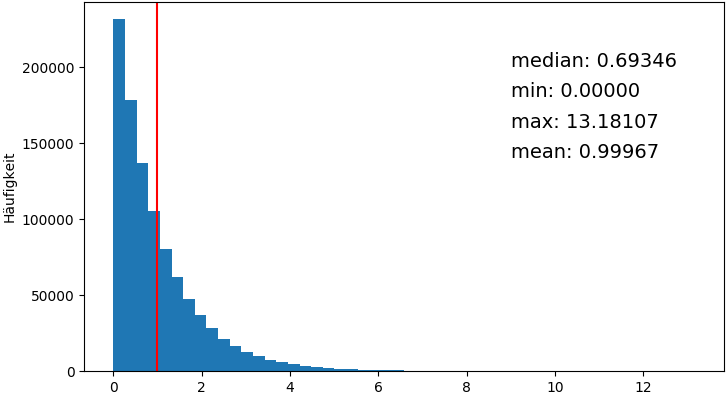
\includegraphics[width=1\textwidth]{pics/negexp.png}
  \caption{Histogramm für die Verteilungsfunktion negexp(1) von Renew nach 1Mio Wiederholungen }
  \label{pic:negexp}
\end{figure}

Wie der Name der Funktion bereits andeutet handelt es sich um eine negativ exponentiell abfallende Funktion. Aus dem gezeigten Graphen lässt sich ablesen das der Eingabewert der Funktion die durchschnittliche Zeit der Ausgabe darstellt. Die Hälfte aller Ausgabewerte ist unter $0.7$ und kompakt auf einer Breite von $0.7$ vertreten, die zweite Hälfte von $0.7$ bis $13.8$ ist wesentlich breiter verteilt mit verschwindend geringer Wahrscheinlichkeit für hohe Werte. 

\begin{figure}[ht]
  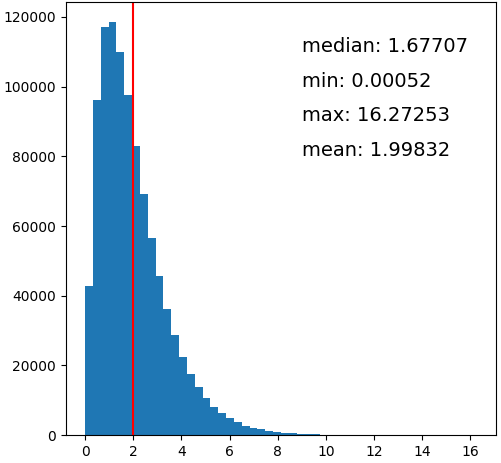
\includegraphics[width=1\textwidth]{pics/negexp2.png}
  \caption{Histogramm für negexp(1) + negexp(1) für 1Mio Wiederholungen}
  \label{pic:negexp2}
\end{figure}

Ähnlich wie bei einem Wurf mehrerer Würfel ergibt sich für die Addition zweiter Funktionsaufrufe ein neuer Peak. Der neue Graph (Abbildung \ref{pic:negexp2}) ist nun nicht mehr konstant fallend sondern steigt zunächst bis auf sein Maximum und fällt danach ab. Ein ähnliches Verhalten wird in der Simulation ebenfalls, bei der Aneinanderreihung der Handlungen der Köche, erwartet. Diese Eigenschaft scheint intuitiv gut geeignet um die Zeit für diesen Prozess zu berechnen da bei der Herstellung eines Gerichtes einerseits Köche verschieden schnell arbeiten, was zunächst für eine Normalverteilung spricht. Allerdings können auch unvorhergesehene Dinge passieren die den Herstellungsprozess stören wie z.B. das sich ein Koch verletzt, Zutaten nicht vorbereitet sind oder ein Koch gerade eine Zigarette rauchen ist. So kann es in Einzelfällen zu wesentlich höheren Herstellungszeiten führen. Mit zunehmender Anzahl von Handlungen wird die Varianz der Zeiten im Verhältnis sinken, denn je mehr Zeiten aufaddiert werden desto geringer ist die Wahrscheinlichkeit das alle Werte sehr hoch oder sehr niedrig werden.

Es muss weiter beachtet werden, dass Handlungen einen minimalen Zeitaufwand haben. Ein Funktionsaufruf von negexp() kann auch einen Wert von 0 zurückliefern und die Handlung so direkt nach Antritt abschließen. Dieses Verhalten ist nicht gewünscht und wird verhindert dadurch, dass eine konstante hinzuaddiert wird, die den minimalen Zeitaufwand darstellt. Eine Zeitfunktion sie dann wie folgt aus

\begin{eqnarray}
	t_{tr_i}  = & t_{tr_{i,1}} \cdot Dist.negexp(t_{tr_{i,2}}) & \\
	t_{tr_i,\mu}  = & t_{tr_{i,1}} +t_{tr_{i,2}}  & \textrm{(Durchschnitt)}\\
	\widetilde{t}_{tr_i}  \approx & t_{tr_{i,1}} + 0.69 \cdot t_{tr_{i,2}} & \textrm{(Median)}
\end{eqnarray}



Für die Entwicklung des neuen timed Net's können die Köche als Ressourcen angenommen werden die jeweils nur von einer Transition zur Zeit genutzt werden können. 

Wenn für alle Transitionen Zeiten hinterlegt sind kann mit den Simulationen begonnen werden. Die Simulationen werden dann für 1,2,3,4 und 6 Köche jeweils einige male wiederholt bis sich ein repräsentatives Ergebnis ablesen lässt.












 %Jan
\section*{Umsetzung} % (fold)
\label{sec:umsetzung}

%% Hier schreiben wie wir das netz gebaut haben


Tabelle \ref{tab:zeiten} zeigt die von uns approximierten Zeiten für die vorhandenen Transitionen. Für alle Handlungen wird davon ausgegangen das die für die Handlung notwendigen Zutaten und Materialien dem Koch direkt vorliegen und der Koch sofort mit dem Vorgang beginnen kann.

\begin{table}[ht]
\centering
\caption{Zeiten für Handlungen/Transitionen}
\vspace{4mm}
\label{tab:zeiten}

	\begin{tabularx}{\textwidth}{| >{\setlength\hsize{\hsize}\centering}X | >{\setlength\hsize{\hsize}\centering}X |}
	\hline
	Handlung / Transition & Zeit in s \tabularnewline \hline \hline
	Vanilleschote aufschneiden & 	3 + Dist.negexp(1) \tabularnewline \hline
    Mark aufkochen & 	180 + Dist.negexp(5) \tabularnewline \hline
    Milch \& Stärke verrühren & 	5 + Dist.negexp(4) \tabularnewline \hline
    Zitrone \& Wein mischen &  5 + Dist.negexp(1) \tabularnewline \hline
    Weinsoße schaumig rühren &  40 + Dist.negexp(5) \tabularnewline \hline
    Milch/Stärke \& Vanillemilch verrühren &  5 + Dist.negexp(1) \tabularnewline \hline
    Vanillecreme aufkochen & 60 + Dist.negexp(10) \tabularnewline \hline
    Vanillecreme abkühlen lassen & 260 + Dist.negexp(40) \tabularnewline \hline
    Ei trennen &  5 + Dist.negexp(1) \tabularnewline \hline
    Eiweiss schlagen &  20 + Dist.negexp(4) \tabularnewline \hline
    Schnee unter Vanillecreme unterheben &  5 + Dist.negexp(5) \tabularnewline \hline
    Vanillecreme + Schnee abfüllen &  2 + Dist.negexp(2) \tabularnewline \hline
    Vanillecreme mit heißer Weinsoße auffüllen &  2 + Dist.negexp(2) \tabularnewline \hline

    \end{tabularx}
\end{table}
Das erweiterte Petrinetz sieht wie in Abbildung \ref{pic:petrinetz} dargestellt aus. Es wurde ein \textit{Hilfs-Platz} namens Tasse hinzugefügt, der dazu dient, dass die Stärke nicht doppelt für die Herstellung von dem Milch-Stärke-Gemisch verwendet wird, und das System verklemmt. Zusätzlich wurde ein Platz namens \textit{Koch} hinzugefügt, der eine Kante zu allen Transitionen die eine Tätigkeit eines Kochs repräsentieren hat. An diesem Platz wird die Anzahl der Köche durch die Startmarkierung verändert.
\begin{figure}[ht]
  \fbox{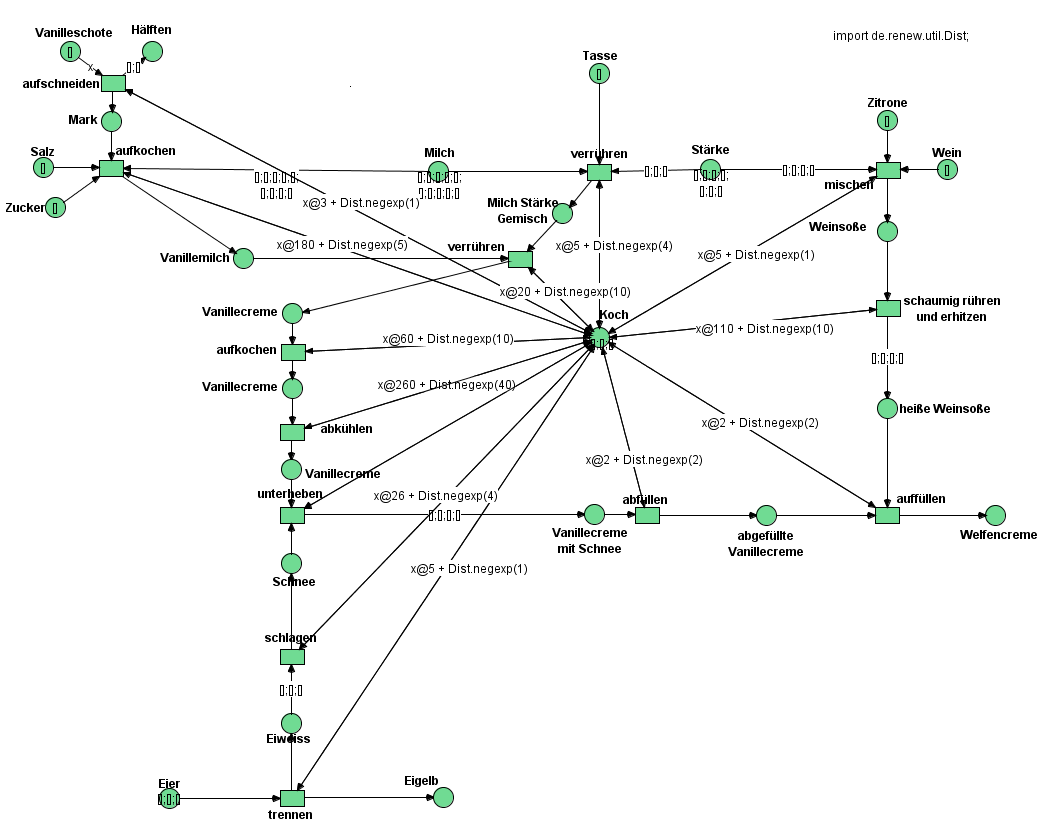
\includegraphics[width=1\textwidth]{pics/net.png}}
  \caption{Das auf Basis der Rezeptur erstellte Petrinetz, erweitert zum timed Net}
  \label{pic:petrinetz}
\end{figure}

Die Durchführung haben wir mithilfe eines von uns geschriebenen Autohotkey-Skripts automatisiert, worüber das Starten und Stoppen getriggert wurde. Die Datenausgabe haben wir über den Start von Renew über den folgenden Aufruf in eine Textdatei schreiben lassen:
\begin{lstlisting}
java -jar loader.jar gui > data.txt
\end{lstlisting}

% section aufgabe_3 (end)
 %Lukas 
\section*{Analyse} % (fold)
\label{sec:analyse}
Das Resultat ist in Abbildung \ref{pic:sim} dargestellt. Die dunkel gestrichelte Linie ist repräsentiert die neunte Dezille bezogen auf die durch die Farbe repräsentierte Anzahl an Köchen. Die zuvor definierte Frage \textit{Wie viele Köche müssen beschäftigt werden damit mindestens 90\% aller Gäste, 10min nach ihrer Bestellung, ihre Welfencreme bekommen?} lässt sich mit \textit{es werden drei Köche benötigt} beantworten.
\paragraph{Beobachtungen}
Aus betriebswirtschaftlicher Sicht ist es evtl. besser sich nur für zwei Köche zu entscheiden, weil der zeitliche Nachteil gegenüber drei Köche nicht groß ist (ungefähr 20 sec. bei der neunten Dezille). Eine weitere interessante Beobachtung ist, dass die größte zeitliche Verbesserung bei dem Sprung von einem auf zwei Köche zu verzechen ist. Der Median sinkt von 866,9 auf 575,5 Sekunden. Betrachtet man dazu im Vergleich die Beschleunigung beim Einsatz von sechs, statt vier Köche, hat man nur eine Verbesserung von ca. zwölf Sekunden im Median.
Dieses Verhalten kann man auch in der IT, beim Einsatz von mehreren Prozessoren beobachten. Sofern die Anwendung nicht auf mehr Prozessoren ausgelegt ist, ist die Performanceverbesserung durch den Einsatz von mehr Prozessoren nur beschränkt. 


\begin{figure}[ht]
  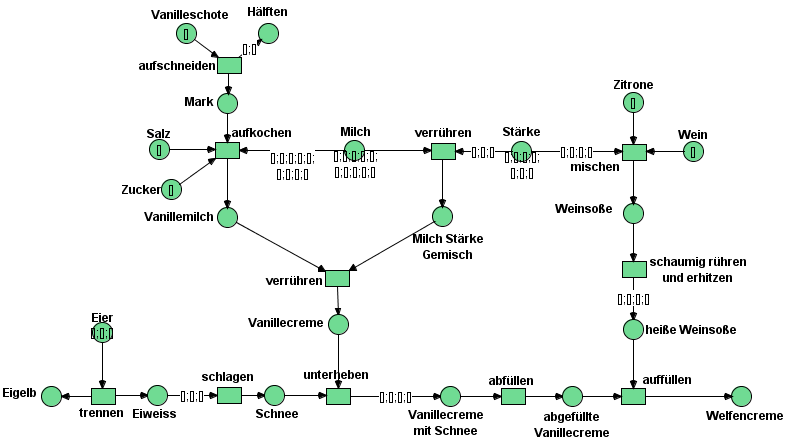
\includegraphics[width=1\textwidth]{pics/sim.png}
  \caption{Histogramm: Die Simulation des Petrinetzes mit verschiedener Anzahl Köchen, gepunktet der korrespondierende Median, dunkel gestrichelt 9. Dezille}
  \label{pic:sim}
\end{figure}


% Wie haben wir die Daten gewonnen ?
% Autohotkey ...
% java -jar loader.jar gui > data.txt

%Denk an die Fragestellung die ich aufgestellt habe und sag in wie weit die Ergebnisse auf eine reale Arbeitsumgebung anwendbar sind (nur bedingt ...)

% 9. Dezille heißt, dass 90% der Werte unterhalb dieses Wertes liegen und 10% drüber -> Fragestellung
 %Lukas


%\nocite{*}
%\bibliographystyle{IEEEbib}
%\bibliography{biblio}
%\clearpage
%\addtocmark[2]{Author Index} % additional numbered TOC entry
\renewcommand{\indexname}{Author Index}
\printindex
\end{document}
